\documentclass[12pt]{sotsuron}
\usepackage{graphicx}
\usepackage{wrapfig}

\title{患者が主体となった医療情報データベースシステムの開発}
\etitle{Development of medical information database
system the patient has become the subject}
\author{松岡 竜嗣}
\teacher{青山 俊弘 准教授}
\date{平成28年1月22日}
\affiliation{電子機械工学専攻}

\begin{document}
\maketitle

\begin{abstract}
This paper presents a web app which can share healthcare
information between patient and doctor.

%\input{abstJapanese}
\end{abstract}

\pagenumbering{roman}
\tableofcontents
\clearpage


\pagenumbering{arabic}

\section{はじめに}
 医療の連携はうまくいっていない.ICTでいいかんじにやろうと国主体でやってるが,いまいち.あじさいネットは成功例.でも全国に普及してるわけではない.\cite{bibi3}
 共通の規格が活用されていない現実があるので,いろんな規格の差を吸収できるようなアプリは需要があるんじゃないかな.とりあえずシェアが大きそうなss-mixを中心に
 既存アプリid-linなどは患者idをリンクしているだけで情報を一元的に集約はしていない.
 人の生涯よりアプリの寿命の方が短い.アプリに合わせてデータベース設計されてる.NoSQLに普遍的に情報をためてって,時代に合わせたアプリ,ヴューでうまいことやろうぜ.
開発年内に殺す.

\clearpage

\section{関連研究}
\subsection{企業発信の類似製品}
 共通の規格が活用されていない現実があるので,いろんな規格の差を吸収できるようなアプリは需要があるんじゃないかな.とりあえずシェアが大きそうなss-mixを中心に
 既存アプリid-linなどは患者idをリンクしているだけで情報を一元的に集約はしていない.
    あじさいネットは10年にわたる活動の中でアンケートを繰り返し,会費だけで運用することができるシステムになっていった.三重県にこのような医療ネットワークを実現するためのたたき台として本研究では開発を進めた.

\subsection{SQL,NoSQLについて}

\clearpage

\section{目的}
前章のように,日本では医療情報が全ての医療機関では共有されていない.
そこで,
患者が自身の医療情報を操作できて,
異なるフォーマットからの入力に
対応した医療情報を共有するシステムを提案する.
提案システムの設計を図\ref{system_construct},
図\ref{class}の
UMLユースケース図とUMLクラス図によって示す.

\begin{figure}[htbp]
  \begin{center}
    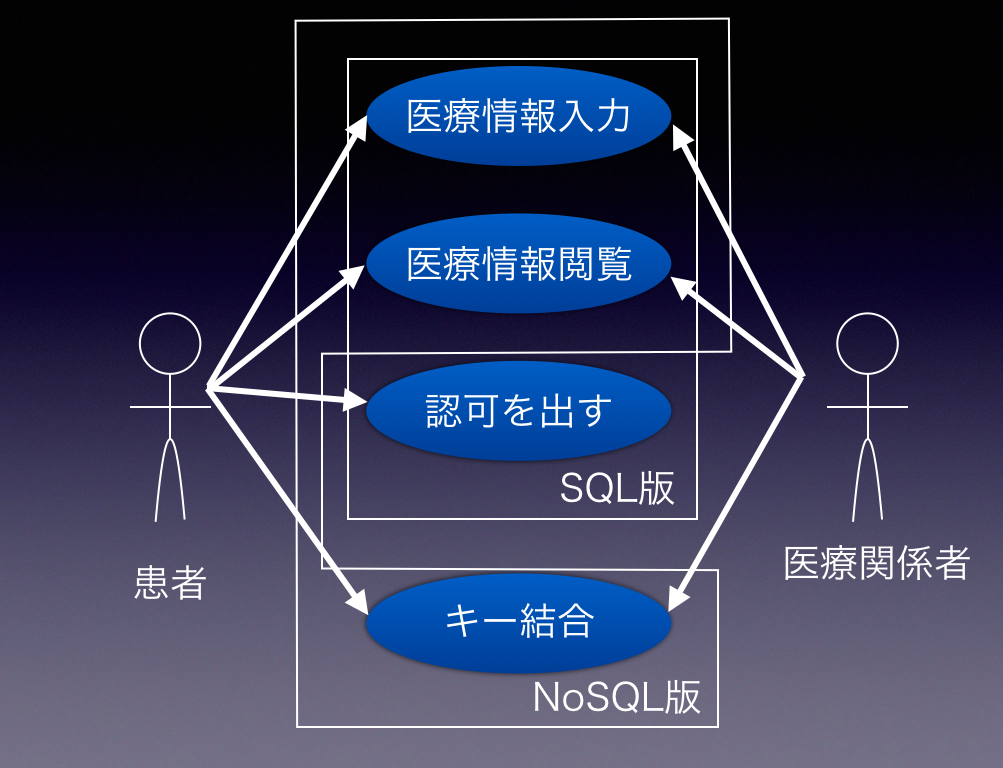
\includegraphics[width=10cm, bb=0 0 1003 768]{./gazou/system_construct2.png}
  \end{center}
  \caption{システムのUMLユースケース図}
  \label{system_construct}
\end{figure}

\begin{figure}[htbp]
  \begin{center}
    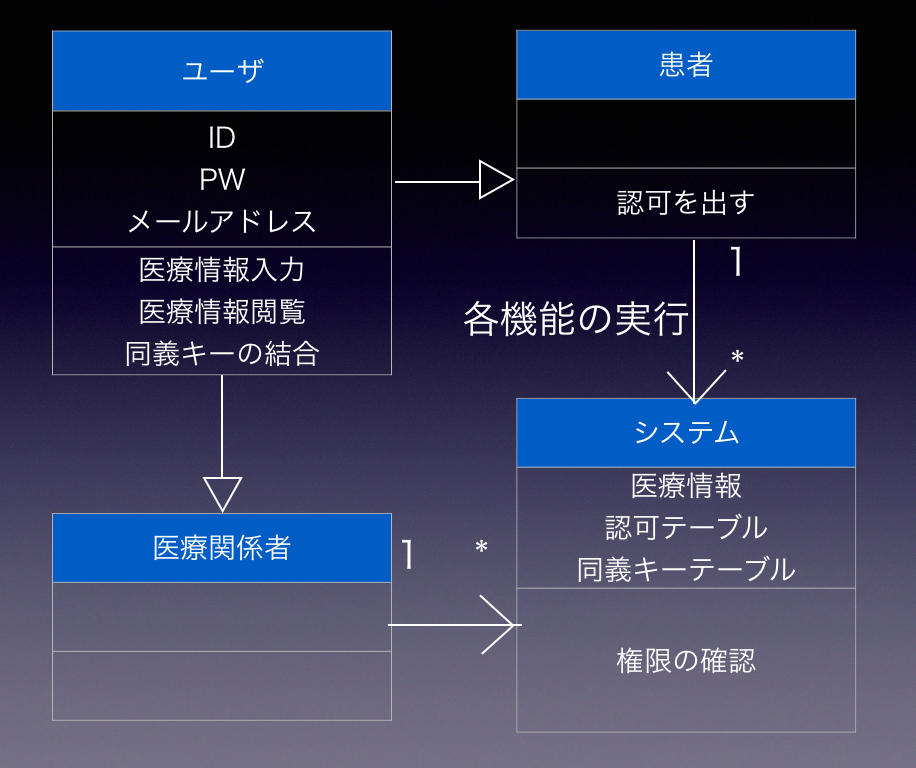
\includegraphics[width=10cm, bb=0 0 916 760]{./gazou/class.png}
  \end{center}
  \caption{UMLクラス図}
  \label{class}
\end{figure}

医療情報の入力と閲覧は既存のシステムにも導入されていて,
医療情報共有システムとして必須と言える.
%SQLデータベースを用いたシステムは医療情報を整形することができたので
%表とガントチャートによって医療情報を出力している.

認可を出す機能は患者が利用できる機能で,
自身の医療情報を操作できる医療関係者を選択するためのものである.

キー結合とはCouchDBを用いたシステムのための機能である.
異なる形式の入力データは同じ意味の項目であっても,
厳密に同じ言葉を項目名にとっていないことがある.
例えば薬を処方した日という意味の項目に対して処方日という項目名と
日時という項目名をとっている場合がある.
CouchDBからデータを抽出する際,これらを同義として抽出できなければ,
データがあるにもかかわらず,診断や処方の際に利用できない.

ここでは便宜的に処方日と日時のように,
異なる項目名であるが同じ意味の項目の群を
同義キーと呼ぶ.
この同義キーを関連付ける機能を実装することで
異なる形式からの入力情報を関連付ける.
具体的な機能として,同義キーのうちのひとつが検索される際に,
その同義キーの群の項目も検索結果として反映させる.

\clearpage

\section{患者が主体の情報共有データベースシステム}
 あじさいネットは10年にわたる活動の中でアンケートを繰り返し,会費だけで運用することができるシステムになっていった.三重県にこのような医療ネットワークを実現するためのたたき台として本研究では開発を進めた.
\clearpage

\section{複数フォーマットに対応した情報共有データベースシステム}
\subsection{アプリケーションの開発環境}
 webアプリケーション開発にはjavascriptのwebフレームワークである
Node.jsを用いた.Node.jsのパッケージであるExpressとnanoを用いた.
Expressはwebフレームワークで、nanoはCouchDBのためのドライバである.
その他に開発で使用したソフトを含めたバージョンなどの情報は付録に記載する.




\subsection{データベースの設計}
	CouchDBにss-mixの仕様書に記載されている
	データ格納方法およびデータ定義\cite{bibi1}に基づいてデータを格納する.
	CouchDBはひとつのデータベースの中に複数のドキュメントとよばれる
	データ構造を保持している.
	このドキュメントは事前にテーブルなどで定義する必要がなく,
	JSON形式であれば自由に記述できる.

	本研究ではひとつの医療行為に対してひとつのドキュメントで管理する.
	本研究で使用するドキュメントが保持する情報を表\ref{tab:doc}に示す.


	\begin{table}[htb]
		\begin{center}
			\caption{ドキュメントが保持する情報}
			\begin{tabular}{|l|c|r|r|}\hline
			Key & Value \\ \hline \hline
			id &  患者名、日付をドキュメントIDとしている. \\ \hline
			rev & \shortstack{ドキュメントの更新回数を示す. \\ 更新時に参照し競合を防ぐ.} \\ \hline
			name & 患者の名前 \\ \hline
			data & \shortstack{医療行為によって得られた情報を \\ json形式で格納.} \\ \hline
			\end{tabular}
			\label{tab:doc}
		\end{center}
	\end{table}


\subsection{アプリケーションの仕様}

	\subsubsection{新規のフォーマットのファイルに対するコスト}
	縦向き、横向きのcsv(地域の病院で生まれるような電子化された医療情報)
	の入力に対応している.
	行と列のどちらかに日付,他方に項目があると想定して入力ファイルから
	医療情報をキーと値に関連付けてデータベースに登録していく.

	電子カルテ固有の出力ファイルはHL7に対応していれば入力ファイルから
	医療情報をキーと値に関連付けてデータベースに登録していく.
	HL7の出力ファイルはパイプ区切りで,データの並び順に意味を持たせている.
	この並び順と項目,データを関連付けてキーと値に置き直して
	データベースに登録していく.

	このとき,HL7のデータの並び順と項目に関する情報が
	アプリケーション側で必要となる.
	つまり,異なる規格の医療情報を登録する際,
	そのフォーマットでデータをどのように意味付けしているかという情報を
	登録するコストが新規のフォーマットのファイルを
	アプリケーションに対応させるためにかかる.


	\subsubsection{同義キーの登録に対するコスト}
	医療情報の出力にはキーを関連付けるためのコストがかかる.
	これは新しいフォーマットで医療情報が入力されるたびに生まれる作業となる.
	これを医療関係者にさせることを想定している.


 %医療情報を収集するNoSQLデータベースシステム.UIとしてWebアプリを用意し,
	%医療関係者,薬剤師,患者の3者に対して,情報を扱いやすいようにした.

\subsection{患者情報閲覧}
	ユーザはログイン後,Accountタブから検索ワードを送信すると,
	/getdbでキーに検索ワードを値に含むキーと値の組を表示する.

	ここで,同義キーで管理されている項目群を表示するために
	キー同士の関連が登録されているドキュメントを参照している.



		\begin{figure}[htbp]
				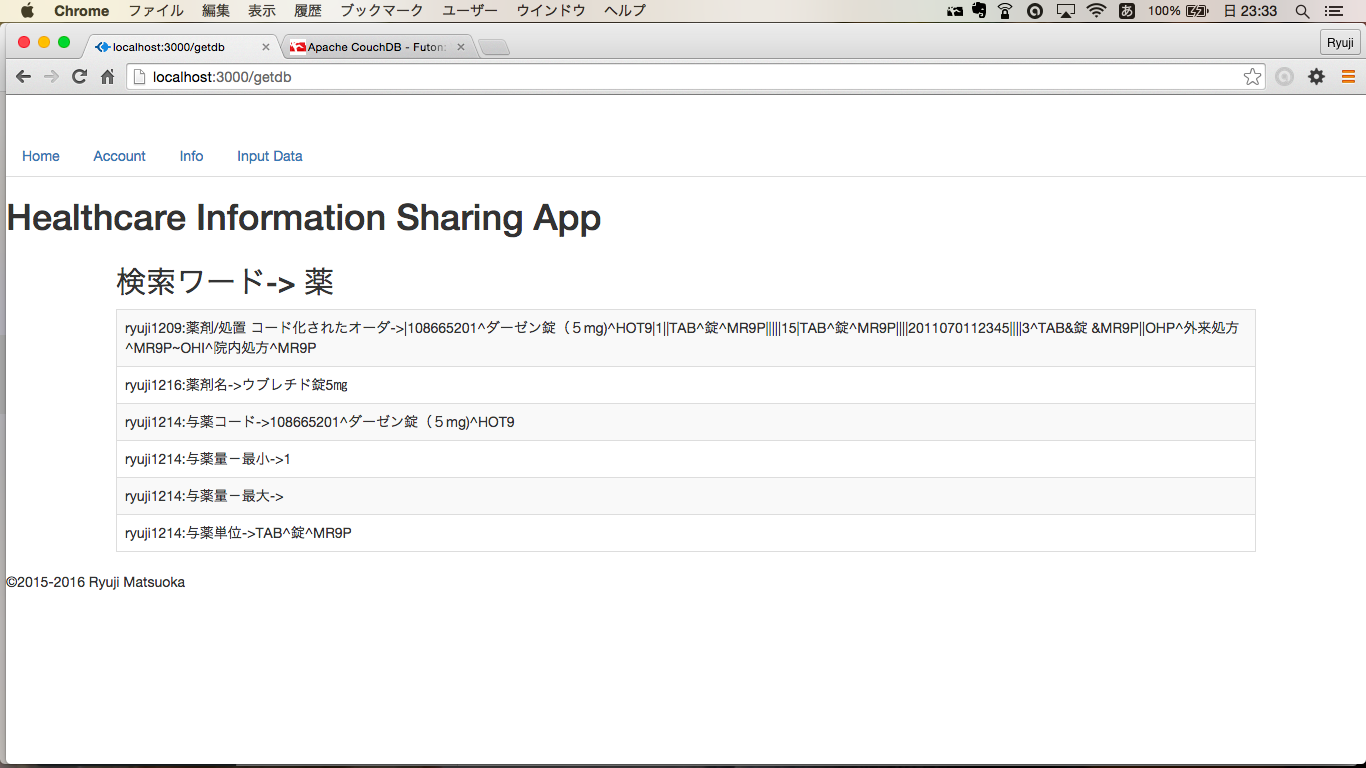
\includegraphics[width=5cm, bb=0 0 437 688]{./gazou/getdb.png}
			\caption{薬 でデータ抽出した様子}
			\label{ss-mix_sampledata}
		\end{figure}



\subsection{データの投入方法}
	ユーザはログイン後,Input Dataタブを選択する.
	次に入力するファイルを選択し,送信する\ref{fileiopage}.

	\begin{figure}[htbp]
		%\begin{center}
			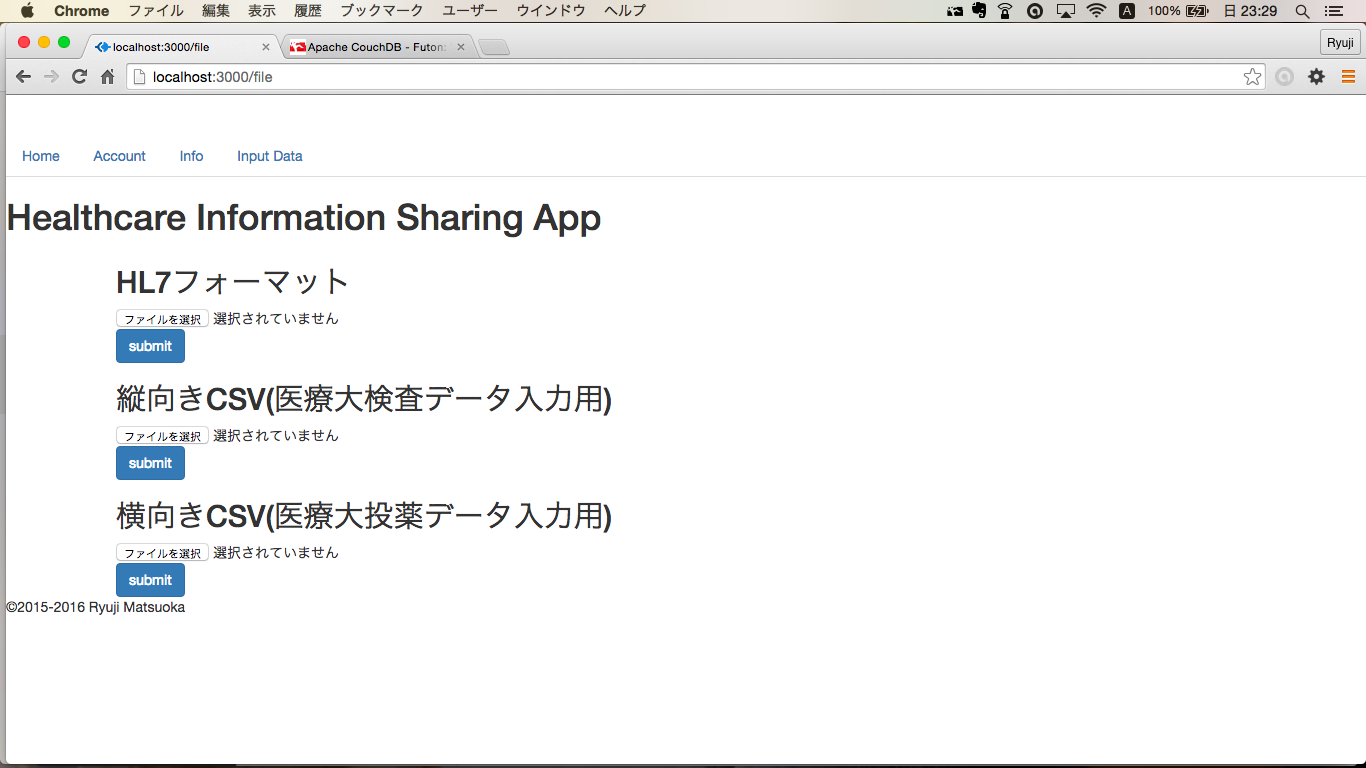
\includegraphics[width=5cm, bb=0 0 437 688]{./gazou/fileiopage.png}
		%\end{center}
		\caption{ファイル入力ページ}
		\label{fileiopage}
	\end{figure}

	1度の診療で1つのドキュメントを生成する.
	CSV入力ファイルに複数回の診療の記録があることを許容する.

		\subsubsection{縦向きcsvファイルの場合}
			parse
			医療大の検査データ
			\\
			\begin{figure}[htbp]
				%\begin{center}
					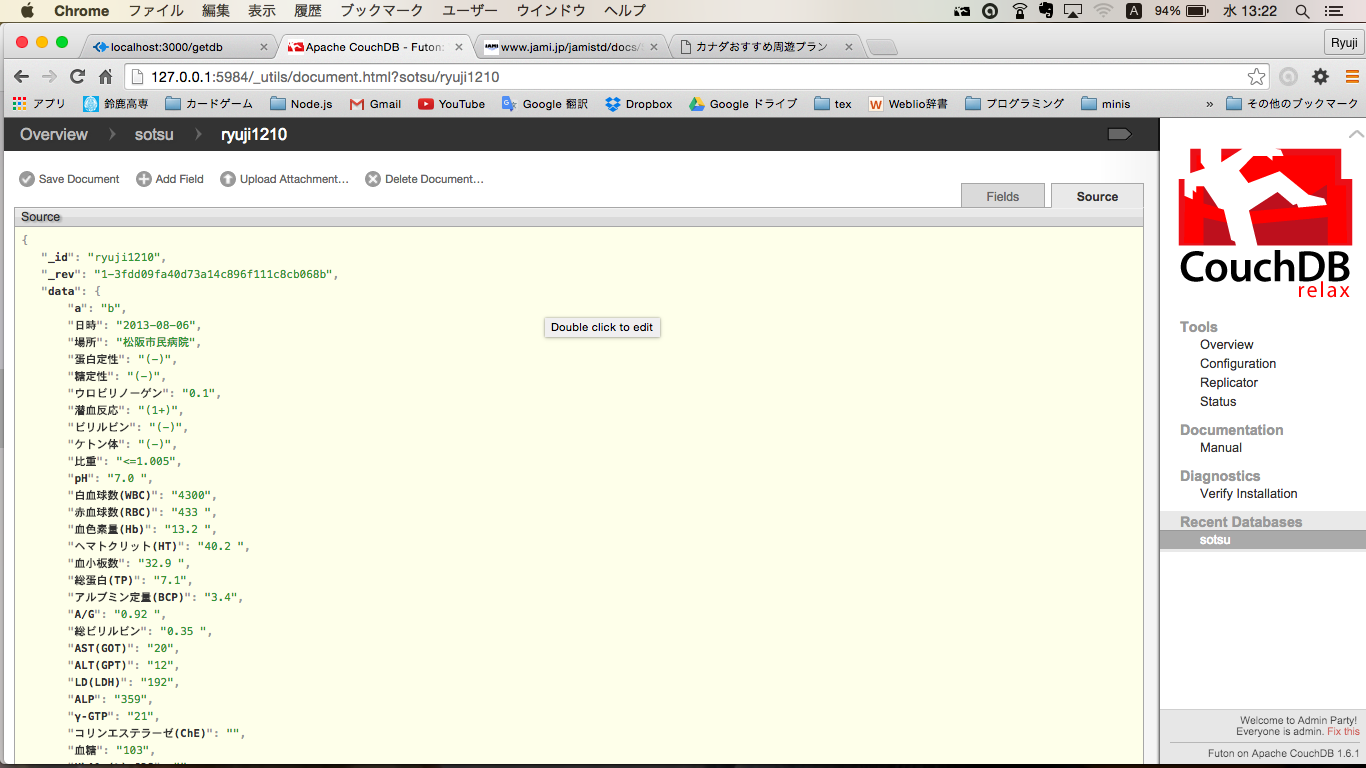
\includegraphics[width=5cm, bb=0 0 437 688]{./gazou/kensa.png}
				%\end{center}
				\caption{医療大の検査データ}
				\label{iryoudai-kensa-data}
			\end{figure}

		\subsubsection{横向きcsvファイルの場合}
			holizontialparse
			医療大の投薬データ
			\\
			\begin{figure}[htbp]
				%\begin{center}
					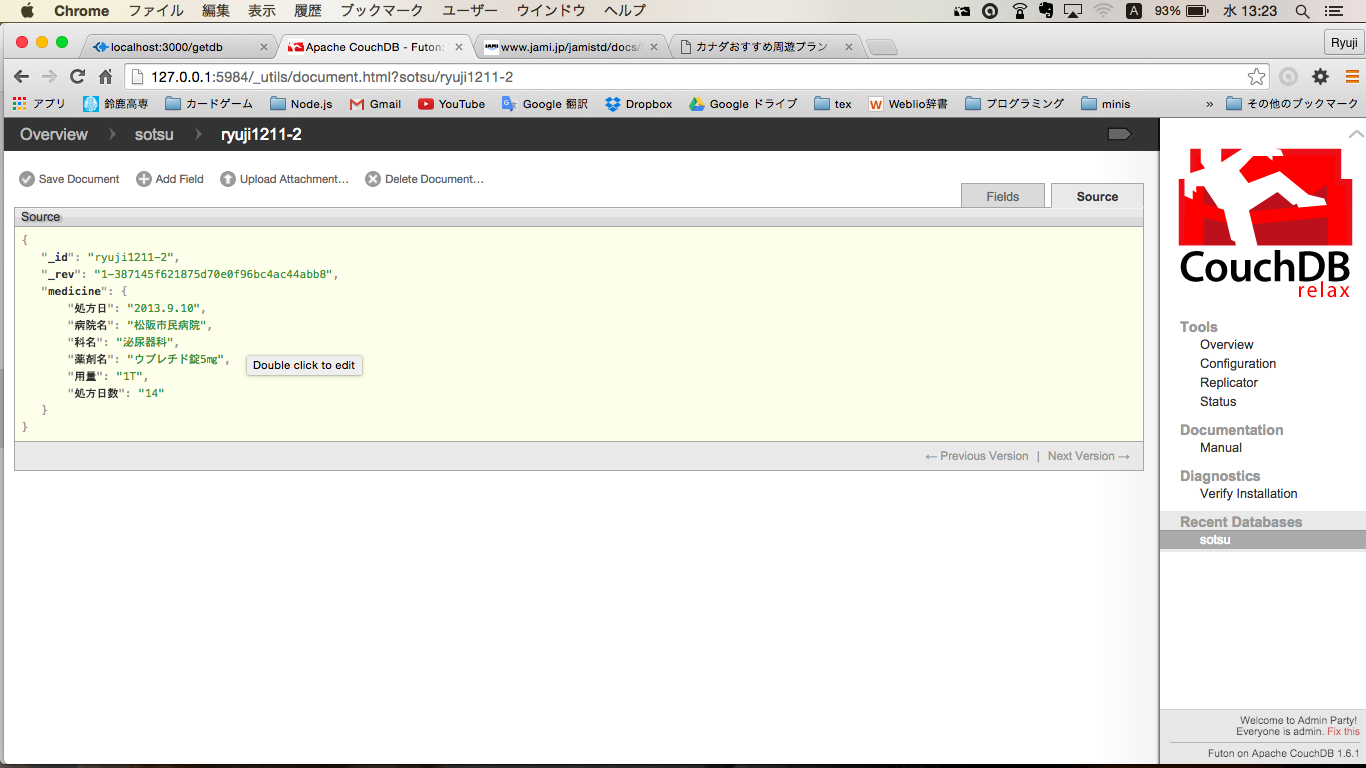
\includegraphics[width=5cm, bb=0 0 437 688]{./gazou/touyaku.png}
				%\end{center}
				\caption{医療大の投薬データ}
				\label{iryoudai-touyaku-data}
			\end{figure}

		\subsubsection{パイプ区切りのHL7ファイルの場合}
			前述のデータ定義に基づいて入力ファイルからデータを格納していく.
			本研究では医療規格にのっとっていない医療情報との関連付けを課題としている.
			そこでHL7にのっとったファイルからデータを抜き出し,
			データの配置によって割り振られている意味をキーとしてデータベースに
			格納していく.

			\begin{figure}[htbp]
				%\begin{center}
					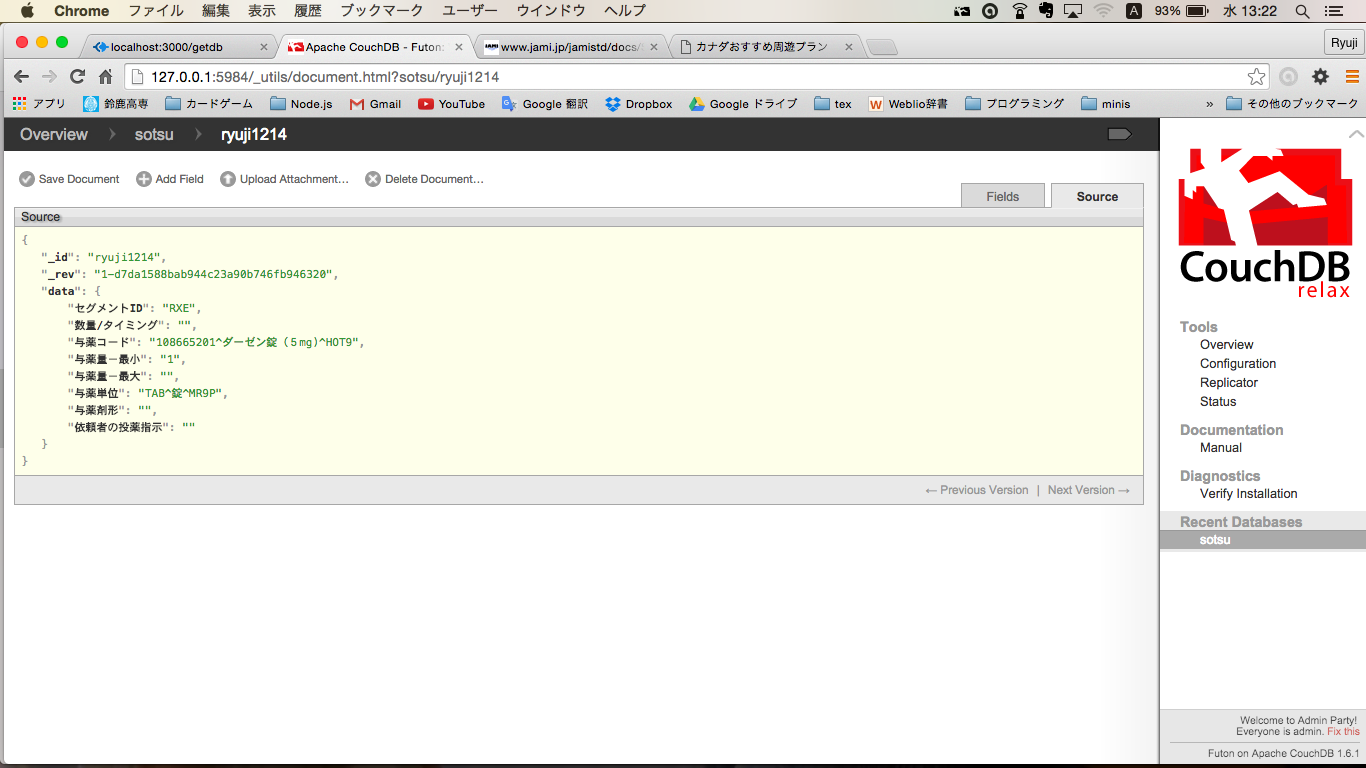
\includegraphics[width=5cm, bb=0 0 437 688]{./gazou/hl7.png}
				%\end{center}
				\caption{HL7のサンプルデータ}
				\label{hl7-data}
			\end{figure}



\subsection{同義キーの登録}
	データを参照するときに,キーが必要となる.キーには様々な意味を持つものがあるが,
	異なる規格のデータでは同じ情報を指し示すキーであっても,
	異なるキーが使われている.
	これは新規の規格が医療情報ソフトに流入するたびに課題となる.

	そこで,本研究ではユーザによる同義キーの登録の機能を用意した.
	ユーザは同義である2つのキーを入力すると
	それが同義キーを管理するドキュメントに追加される.

	図\ref{relation}では投薬データの処方日と診断データの日時が同義として登録されている.
	図\ref{relationApp}では検索ワードは処方であるので
	処方をキーに含むデータが検索結果として表示される.
	さらに,検索結果に処方日があり,これは日時と同義として登録されているため,
	日時のデータも検索結果として表示される.
	(実装まだですが.texが嫌になった時にやります。
	仕様としては、処方日、日時ともにその右に日付がならびます。)

	\begin{figure}[htbp]
		%\begin{center}
			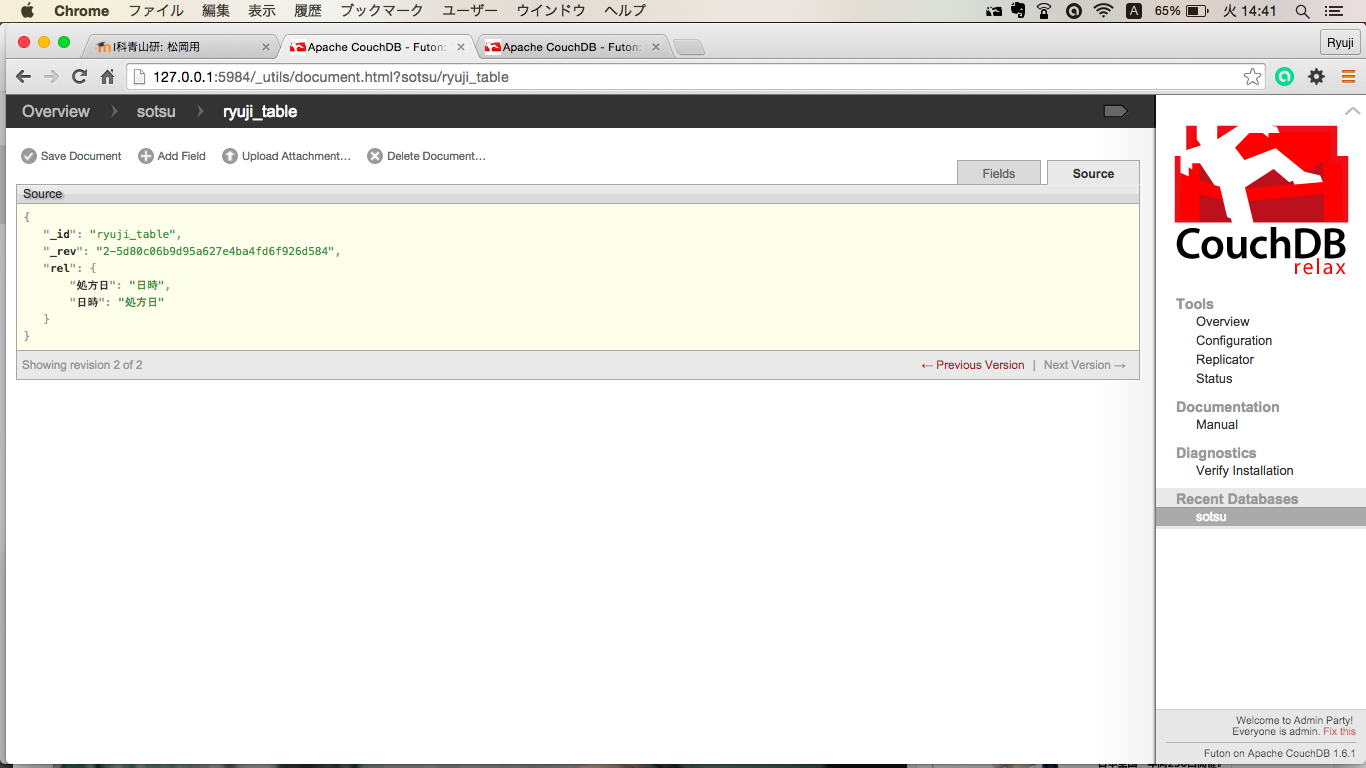
\includegraphics[width=5cm, bb=0 0 437 688]{./gazou/relation.png}
		%\end{center}
		\caption{同義キーを管理するドキュメント}
		\label{relation}
	\end{figure}

	\begin{figure}[htbp]
		%\begin{center}
			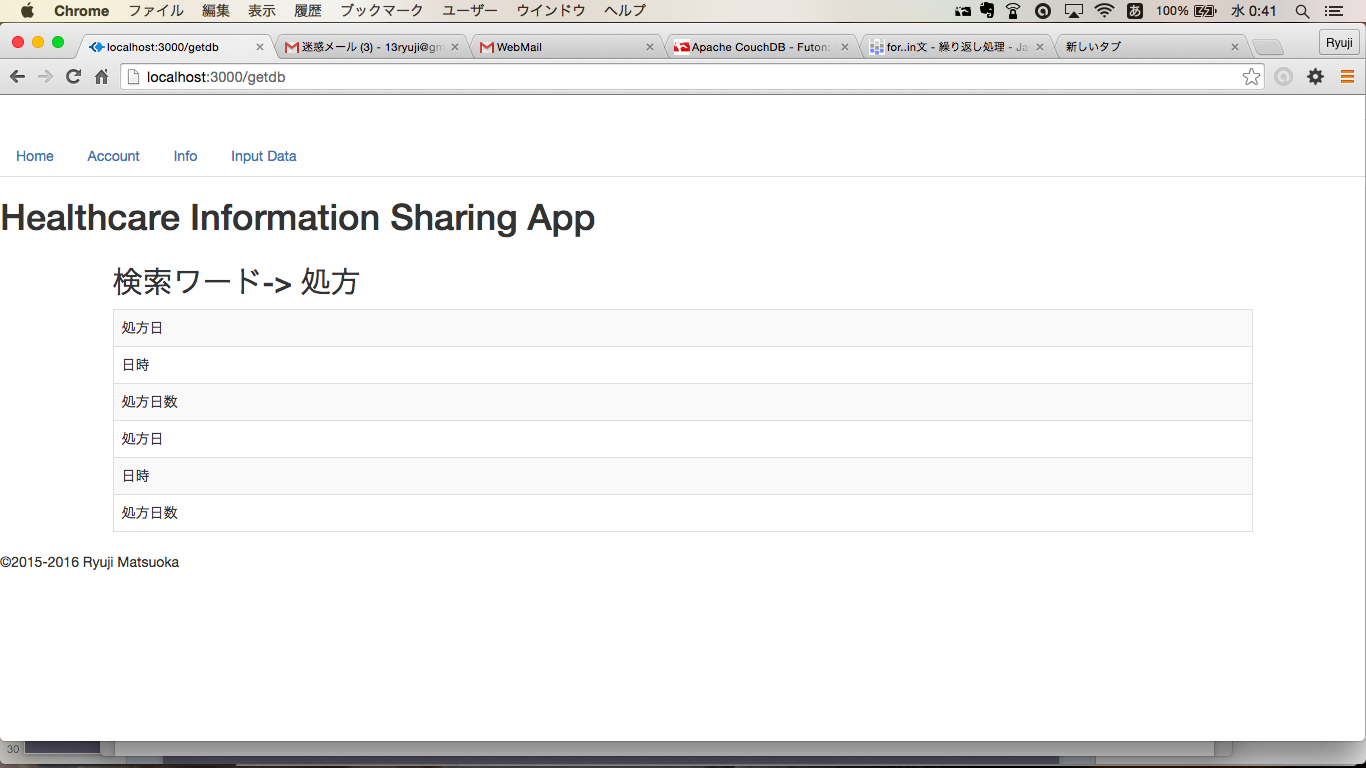
\includegraphics[width=5cm, bb=0 0 437 688]{./gazou/relationApp.png}
		%\end{center}
		\caption{処方と検索して同義キーとして登録されている日時を表示する}
		\label{relationApp}
	\end{figure}

\clearpage



\section{結果・考察}
\subsection{実装した機能とそれによって解決した課題}
  自由に記述されたエクセルファイルと
  入力が想定されている電子カルテの出力ファイルを
  入力ファイルとして受け付けることができた.
  これにより,統一規格が整備されていない
  医療情報であっても一元的に収集することができると言える.
  ここで,エクセルファイルでは行か列のどちらかに項目があることを
  前提としているので完全に自由とは言えない.
  しかし,エクセルファイルで複数の項目やデータを扱う場合には
  日常的に行か列のどちらかに項目を入力するので
  これは制限にならないと考えられる.

  様々なフォーマットによって入力された医療情報を
  関連付けて活用するために同義キーの登録機能を実装した.
  これにより,同じ意味の項目がフォーマットの都合によって
  消されることなく扱うことができる.

  患者に認可の権限を与えることで,患者の心的負担を軽減することができる.


%\subsection{運用に向けて}
  \if0
  \subsubsection{ユーザアカウントの管理方法}
    患者の電子カルテは病院ごとのIDで管理されているので,
    病院ごとのIDを特定の患者アカウントに対して
    結びつける必要がある.

    また,患者が医療関係者に対して与える認可の範囲において,
    本研究では医師一人に対して権限を与えているが
    その医師が所属する機関に同様の権限を与えるべきかどうか
    検討している.
  \fi

\subsection{データの信頼性}
  %\subsubsection{データの信頼性}
    入力された医療情報はデータを採取した人物や機器の違いを考慮していない.
    これらの差を考慮する必要が出たとき,
    NoSQL版のデータベース内のドキュメントに
    新たな項目を追加することで対応することができる.
    しかし,誰が入力したかを明記して医療情報の共有を行うことは
    医療関係者の心理的負担になることが海外の先行研究から分かっている.
    \cite{bibi10}

%  \subsubsection{データの暗号化}
%    プロトタイプ開発のため,データの保護に関する

\if0
---以下メモ---
企業製品に対する刺激になるといいな
医療関係者内のお金がらみの事情
   毎回検査したほうが病院は儲かる.
実装もっと力入れるべきだった
    SQLver.で実装できてるグラフやガントチャートをNoSQLver.でも使えたらかっこよかった.
実用化にはセキュリティまわりなど課題多し
\fi

\subsection{本研究の意義}
  本研究では国内で規格の統一化が進まない
  医療情報を収集するデータベースシステムと
  それを共有するためのWebアプリケーションの開発を行った.


  ID-Linkでは各病院の患者の電子カルテのIDを関連付けることで,
  あじさいネットでは参照サーバを介して
  電子カルテの情報を参照するだけに留まっている.
  SS-MIXは医療情報を収集するが,患者自身が医療情報を閲覧したり,
  バイタルを追記したりすることはできない.

  提案システムは患者の認可を得ていることを前提に
  患者と医療関係者の間で共有することができるので
  類似製品や活動よりも医療の質の向上を図れると考えられる.

  NoSQL版はSQL版に比べて医療情報の可視化までに
  内部的な処理が増えるが,
  医療情報の形式のばらつきに柔軟に対応させることができた.


  %医療情報の電子化,共有は方針が定まらず,規格を選定している段階にある.
  %今後, 規格が定まった際に
  %多様な規格の元で生成される医療情報を現段階から収集しておけば
  %有効活用できると考えられる.

\clearpage


\appendix

%\section*{謝辞}
%本研究の遂行,論文作成にあたり,
%多大なご指導を賜りました鈴鹿工業高等専門学校電子情報工学科
%青山俊弘准教授に心から感謝致します.
%また,研究を共にした青山研究室のみなさまにも感謝致します.

\section*{付録}
\begin{table}[htb]
	\begin{tabular}{|l|c|r|r|}\hline
	導入ソフト & バージョン \\ \hline \hline
	Node.js & 0.12.6 \\ \hline
	Express & 4.12.1 \\ \hline
	Passport & 0.3.2 \\ \hline
	passport-hash & 0.5.0 \\ \hline
	connect-flash & 0.1.1 \\ \hline
	Jade & 1.11.0 \\ \hline
	multer & 1.1.0  \\ \hline
	ya-csv & 0.9.4 \\ \hline
	%ya-csv & 0.9.4 \\ \hline
	nano & 6.1.5 \\ \hline
	crypto & 0.0.3  \\ \hline


	\end{tabular}
\end{table}





\begin{thebibliography}{12}
	%背景
	\bibitem{bibi2} 国立病院機構における診療情報分析システムについて・川島直美ら,情報処理学会デジタルプラクティス2013年15号


	%HL7
	\bibitem{bibi5} 日本HL7協会ホームページ,http://www.hl7.jp
  \bibitem{bibi6} 第13回HL7セミナー HL7入門,http://www.hl7.jp/docs/seminar/SeminarNo13Kawamata.pdf

	%ID-Link
  \bibitem{bibi12} ID-Link mykarte.com|地域医療連携ネットワークサービス|株式会社エスイーシー,www.mykarte.org/idlink/


	%SS-MIX
	\bibitem{bibi1} SS-MIX2標準化ストレージ仕様書Ver.1.2c・日本医療情報学会
	\bibitem{bibi7} SS-MIX 普及推進コンソーシアム,http://www.ss-mix.org/cons/



	%あじさいネット
	\bibitem{bibi3} 地域医療連携ネットワークの構築と運用継続性の追求・石黒満久

	%開発
  \bibitem{bibi8} LLフレームワークBOOKS Django×Python・露木誠,技術評論社
  \bibitem{bibi9} はじめてのNode.js-サーバサイドJavaScriptで Webアプリを開発する・松島浩道,ソフトバンク クリエイティブ株式会社

	%プライバシー
  \bibitem{bibi10} Perera, Gihan, et al. "Views on health information sharing and privacy from primary care practices using electronic medical records." International journal of medical informatics 80.2 (2011): 94-101.

	%クラウド
	%\bibitem{bibi11} Vinutha.S, C.K.Raju, Dr.M.Siddappa, "Development of Electronic Hospital Management System utilizing Cloud Computing and Android OS using VPN connections."

\end{thebibliography}


\clearpage

\listoffigures
\clearpage

\listoftables
\clearpage


\end{document}
